\documentclass[12pt, a4paper]{article}
\usepackage[print,sort]{standalone}
\usepackage[T1]{fontenc}
\usepackage[utf8]{inputenc}
\usepackage[english]{babel}
\usepackage{graphicx,float}
\usepackage{amssymb}
\usepackage{amsmath,cancel}
\usepackage{mathrsfs}
\usepackage{epstopdf}
\usepackage{subcaption}
\usepackage{slashed}
\usepackage{hhline}
\usepackage[margin=1.2in]{geometry}
\usepackage[hidelinks]{hyperref}
\usepackage{wrapfig}


\hfuzz=5pt


\begin{document}

\begin{titlepage}
\begin{center}
\vspace*{3cm}
\Huge
\textbf{Project 2} \\
\Large  
FYS4150 Computational Physics 
\vspace*{3cm} \\ 

Even S. Håland 
\vspace*{5cm} \\

\normalsize
\section*{Abstract}


\end{center}
\end{titlepage}

\section{Introduction}

The purpose of this project is to develop a program for solving eigenvalue problems by using Jacobi's 
algorithm. 

\section{The Schrödinger equation}

(This section follows very closely the theoretical introduction given project description, but 
for completeness sake I thought it would be nice to also include it in the report.) 

\subsection{One-particle case}

We start by considering the radial part of the Schrödinger equation (SE) for one electron, which is 
given as 
\begin{align}
- \frac{\hbar^2}{2m}\left( \frac{1}{r^2} \frac{d}{dr}r^2 \frac{d}{dr} - \frac{l(l+1)}{r^2} \right) R(r) 
+ V(r) R(r) = ER(r),
\label{eq:SE}    
\end{align}    
where (in our case) $V(r)$ is the harmonic oscillator (HO) potential 
\begin{align*}
V(r) = \frac{1}{2} k r^2, 
\end{align*}
where $k = m\omega^2$. $E$ is then the energy of the three dimensional HO, $\omega$ is the 
oscillator frequency, and these quantities are related by 
\begin{align*}
E_{nl} = \hbar \omega \left( 2n + l + \frac{3}{2} \right), 
\end{align*}
where $n = 0,1,2,\dots$ and $l = 0,1,2,\dots$. Throughout this project only cases with $l = 0$ will be 
considered. 

By making the substitution $R(r) = (1/r)u(r)$ and introducing the dimensionless variable 
$\rho = (1/\alpha)r$ eq. (\ref{eq:SE}) can be simplified to 
\begin{align*}
-\frac{\hbar^2}{2m\alpha^2} \frac{d^2}{d\rho^2}u(\rho) + \frac{k}{2}\alpha^2 \rho^2 u(\rho) = Eu(\rho),  
\end{align*} 
with boundary conditions $u(0) = u(\infty) = 0$. 
Further we can multiply the equation by $2m\alpha^2/\hbar^2$, and fix $\alpha$ so that 
\begin{align*}
\frac{mk}{\hbar^2}\alpha^4 = 1.  
\end{align*}
If we also define 
\begin{align*}
\lambda = \frac{2m \alpha^2}{\hbar^2}E 
\end{align*}
we end up with the eigenvalue equation 
\begin{align}
- \frac{d^2}{d\rho^2}u(\rho) + \rho^2u(\rho) = \lambda u(\rho). 
\label{eq:SE_1p_scaled}
\end{align}

We must of course make a discrete approximation to the equation in order to solve the problem numerically. 
However, before moving on to that we should have a quick look at the changes that are introduced by 
adding a second electron to the problem. 

\subsection{Two-particle case}

The radial SE for two electrons in an HO potential without any interactions is given by 
\begin{align}
\left( - \frac{\hbar^2}{2m}\frac{d^2}{dr_1^2} - \frac{\hbar^2}{2m}\frac{d^2}{dr_2^2} 
	   + \frac{1}{2}kr_1^2 + \frac{1}{2}kr_2^2 \right) u(r_1, r_2) = E^{(2)}u(r_1, r_2), 
\label{eq:SE_2p_NoInt}
\end{align}
where $E^{(2)}$ is the two-electron energy. The solution to this equation is just the product of the 
wave functions for each electron. However, when we introduce the Coulomb interaction (which depends on 
the distance $r$ between the electrons) eq. (\ref{eq:SE_2p_NoInt}) is not very useful. For that reason 
we would like to introduce a new set of coordinates, namely the relative distance between the electrons,  
\begin{align*}
\mathbf{r} = \mathbf{r}_1 - \mathbf{r}_2, 
\end{align*} 
and the centre-of-mass coordinate for the system, 
\begin{align*}
\mathbf{R} = \frac{1}{2}(\mathbf{r}_1 + \mathbf{r}_2). 
\end{align*}
The SE (still without interactions) can then be written as 
\begin{align*}
\left( - \frac{\hbar^2}{m}\frac{d^2}{dr^2} - \frac{\hbar^2}{4m}\frac{d^2}{dR^2} 
	   + \frac{1}{4}kr^2 + kR^2 \right) u(r,R) = E^{(2)}u(r,R),  
\end{align*}
where $r=|\mathbf{r}_1 - \mathbf{r}_2|$ and $R = \frac{1}{2}|\mathbf{r}_1 + \mathbf{r}_2|$. We then 
assume that the wave function is separable, so that $u(r,R) = \psi(r)\phi(R)$, and that the total energy 
is given by the sum of relative energy, $E_r$, and centre-of-mass energy, $E_R$, i.e. 
\begin{align*}
E^{(2)} = E_r + E_R. 
\end{align*}
We can then add the term for the Coulomb interaction, which is given by 
\begin{align*}
V(r) = \frac{\beta e^2}{r}, 
\end{align*}
where $\beta e^2 = 1.44$ eVnm, and the $r$-dependent part of the SE becomes 
\begin{align*}
\left( - \frac{\hbar^2}{m}\frac{d^2}{dr^2} + \frac{1}{4}kr^2 + \frac{\beta e^2}{r} \right) \psi(r) 
= E_r \psi(r).  
\end{align*}

As we did for the one-electron SE we now introduce the dimensionless variable $\rho = r/\alpha$, and 
scale the equation appropriately. After a few steps of manipulation we arrive to   
\begin{align}
- \frac{d^2}{d\rho^2} \psi(\rho) + \omega_r^2 \rho^2 \psi(\rho) + \frac{1}{\rho} = \lambda \psi(\rho), 
\label{eq:SE_2p_scaled}
\end{align}
where 
\begin{align*}
\omega_r^2 = \frac{1}{4}\frac{mk}{\hbar^2}\alpha^4, 
\end{align*}
with $\alpha$ fixed so that 
\begin{align*}
\frac{m \alpha\beta e^2}{\hbar^2} = 1, 
\end{align*}
and $\lambda$ is defined as  
\begin{align*}
\lambda = \frac{m\alpha^2}{\hbar^2}E. 
\end{align*}

It is noteworthy that the only differences between equations (\ref{eq:SE_1p_scaled}) and 
(\ref{eq:SE_2p_scaled}) is the factor $\omega_r^2$ in the HO potential term, and the Coulomb repulsion 
term. This means that it is quite easy to make the transition between these cases when writing the code, 
which is in fact the main point of doing the scaling.    

\subsection{Discrete Schrödinger equation}

As mentioned previously we must make a discrete approximation to the SE, and when doing so we will jump 
back to the one-electron problem, i.e. eq. (\ref{eq:SE_1p_scaled}). 

The second derivative is approximated (up to $O(h^2)$) by 
\begin{align*}
u'' \approx \frac{u(\rho + h) - 2u(\rho) + u(\rho - h)}{h^2},  
\end{align*}
where $h$ is the step length. The minimum value of $\rho$ is $\rho_{min} = \rho_0 = 0$, while the 
maximum value is in principle infinity. However, infinity is not a very practical ''value'' to work with,
especially in a numerical context, which means that we must choose an appropriate maximum value 
$\rho_{max} = \rho_N$. The step length $h$ is then defined as 
\begin{align*}
h = \frac{\rho_N - \rho_0}{N}, 
\end{align*} 
where $N$ is the number of mesh points we consider, and $\rho$ is given as 
\begin{align*}
\rho_i = \rho_0 + ih, 
\end{align*}
with $i = 1,2,\dots,N$. By using the short-hand notation $u(\rho_i + h) = u_{i+1}$, we can write the 
SE as 
\begin{align}
- \frac{u_{i+1} - 2u_i + u_{i-1}}{h^2} + V_iu_i = \lambda u_i, 
\end{align}
where $V_i = \rho_i^2$ is the HO potential. This is now an eigenvalue problem which can be compactly 
written as $\mathbf{Au} = \lambda\mathbf{u}$, where $\mathbf{A}$ is a matrix with diagonal elements 
\begin{align*}
d_i = \frac{2}{h^2} + V_i
\end{align*}
and non-diagonal elements 
\begin{align*}
e_i = -\frac{1}{h^2}. 
\end{align*} 

If we instead want to consider the two-electron case with the Coulomb interaction we simply change 
the potential $V_i$ from $\rho_i^2$ to $\omega_r^2\rho_i^2 + 1/\rho_i$. 

\section{Jacobi's method}

To summarize the situation we have now reduced the Schrödinger equation to an eigenvalue problem of 
the form $\mathbf{Au} = \lambda\mathbf{u}$, with $A\in \mathbb{R}^{n\times n}$. Our task is then to find 
the $n$ eigenvectors ($\mathbf{u}_1, \mathbf{u}_2,\dots,\mathbf{u}_n$) and eigenvalues 
($\lambda_1,\lambda_2,\dots,\lambda_n$) of $A$. 

The idea behind Jacobi's method is to do a series of orthogonal transformations of the kind 
\begin{align*}
(\mathbf{SAS}^T)(\mathbf{Sv}_i) = \mathbf{Sv}_i, 
\end{align*}
where $\mathbf{S}$ is an orthogonal matrix satisfying $\mathbf{SS}^T = \mathbf{I}$, and $\mathbf{v}_i$ is 
an orthogonal basis of $\mathbb{R}^n$. Our goal is then to eventually end up with a matrix on the 
left-hand side where all non-diagonal elements are (close to) zero, which means that the elements on the 
diagonal are (close to) the eigenvalues. 

This method works because when we do an orthogonal transformation 
\begin{align*}
\mathbf{B} = \mathbf{SAS}^T, 
\end{align*}
the eigenvalues of $\mathbf{B}$ are the same as those of $\mathbf{A}$, and
 it can be shown that \cite{Matrix Comp} if $\mathbf{A}$ is real and symmetric
(which it is in our case) there exists an orthogonal matrix, $\mathbf{M}$, such that 
\begin{align*}
\mathbf{MAM}^T = diag(\lambda_1,\dots,\lambda_n).  
\end{align*} 
(A more careful discussion of this is found in for example refs. \cite{Matrix Comp, Lecture Notes}.) 

We can also see that if the basis vectors, $\mathbf{v}_i$, are orthogonal, that is\footnote{This relation 
actually states that the $\mathbf{v}_i$'s are \textit{orthonormal}, and not just orthogonal.} 
\begin{align*}
\mathbf{v}_j^T\mathbf{v}_i = \delta_{ij}, 
\end{align*}
then after an orthogonal transformation 
\begin{align*}
\mathbf{w}_i = \mathbf{Sv}_i,  
\end{align*} 
the dot product of the new vectors is 
\begin{align*}
\mathbf{w}_j^T\mathbf{w}_i & = (\mathbf{Sv}_j)^T \mathbf{Sv}_i \\
						   & = \mathbf{v}_j^T\mathbf{S}^T \mathbf{Sv}_i \\ 
						   & = \mathbf{v}_j^T\mathbf{v}_i \\ 
						   & = \delta_{ij}, 
\end{align*}
which means that orthogonality (and the dot product) is preserved by orthogonal transformations. This 
provides us with a nice way of testing our algorithm. 

The next step is to choose a basis, $\mathbf{v}_i$, and a transformation matrix, $\mathbf{S}$. The basis 
vectors are chosen as simply as possible, namely 
\begin{align*}
v_1 = \left( \begin{array}{c}
1 \\ 0 \\ 0 \\ \vdots \\ 0
\end{array} \right), \quad 
v_2 = \left( \begin{array}{c}
0 \\ 1 \\ 0 \\ \vdots \\ 0
\end{array} \right), \dots, \quad
v_n = \left( \begin{array}{c}
0 \\ 0 \\ \vdots \\ 0 \\ 1
\end{array} \right),  
\end{align*}
where each vector (of course) has $n$ elements. The transformation matrix is chosen to be the matrix that 
rotates our system by an angle $\theta$ in a plane in the $n$-dimensional Euclidean space. Such a matrix 
has elements 
\begin{align*}
s_{kk} = s_{ll} = \cos\theta, \: s_{kl} = - s_{lk} = -\sin\theta, \: s_{ii} = 1, 
\end{align*}   
where $i \neq k,l$, and for a specific rotation $k$ and $l$ are fixed numbers. All other elements of 
$\mathbf{S}$ are zero. So when doing the transformation 
\begin{align*}
\mathbf{B} = \mathbf{SAS}^T, 
\end{align*}   
the matrix $\mathbf{B}$ gets the following elements: 
\begin{align*}
b_{ii} & = a_{ii},\: i\neq k,l \\
b_{ik} & = a_{ik}\cos\theta - a_{il}\sin\theta, \: i\neq k,l \\
b_{il} & = a_{il}\cos\theta + a_{ik}\sin\theta, \: i\neq k,l \\
b_{kk} & = a_{kk}\cos^2\theta -2a_{kl}\cos\theta\sin\theta + a_{ll}\sin^2\theta \\
b_{ll} & = a_{ll}\cos^2\theta +2a_{kl}\cos\theta\sin\theta + a_{kk}\sin^2\theta \\
b_{kl} & = b_{lk} = (a_{kk} - a_{ll})\cos\theta\sin\theta + a_{kl}(\cos^2\theta - \sin^2\theta)
\end{align*}  
Since we eventually want all the non-diagonal elements to be zeros (within some tolerance) we should chose 
the angle $\theta$ so that $b_{kl} = b_{lk} = 0$. From the expression for $b_{kl}$ above we can get the 
second order equation 
\begin{align*}
\tan^2\theta + 2\tan\theta\tau -1 = 0, 
\end{align*}
where $\tau = (a_{ll}-a_{kk})/2a_{kl}$, which has the roots 
\begin{align*}
\tan\theta = - \tau \pm \sqrt{1 + \tau^2}. 
\end{align*}
By using the relations 
\begin{align*}
\tan\theta = \frac{\sin\theta}{\cos\theta} \quad \mbox{and} \quad \cos^2\theta + \sin^2\theta = 1, 
\end{align*}  
we find that 
\begin{align*}
\cos\theta = \frac{1}{\sqrt{1+t^2}} \quad \mbox{and} \quad \sin\theta = \cos\theta\tan\theta, 
\end{align*}  
which we then apply to our matrix.   
  
For every transformation we do we want to reduce the off-diagonal norm, defined as  
\begin{align*}
\mbox{off}(A) = \sqrt{\sum_i \sum_j |a_{ij}|^2},\quad i\neq j, 
\end{align*}    
such that 
\begin{align*}
\mbox{off}(B) < \mbox{off}(A), 
\end{align*}  
and that this norm in the end should be approximately zero. To reduce the off-diagonal norm as much as 
possible we start each iteration by picking out the largest off-diagonal element, and hence determine 
the indices $k$ and $l$.       
  
\section{Programs and implementation}

All code written for the project can be found in the following git-repository:  \vspace{0.5cm} \\ 
\fbox{
\href{https://github.com/evensha/FYS4150/tree/master/Project2/Programs}
{https://github.com/evensha/FYS4150/tree/master/Project2/Programs} 
} \vspace{0.5cm} \\ 
The code is mainly written in C$++$, while some plotting is done with python. The script which are 
relevant (and will be discussed in the following) are 
\begin{itemize}
\item \texttt{Jacobi\_algorithm.cpp}
%\item \texttt{Jacobi\_algorithm.h}
\item \texttt{Project2.cpp} 
\item \texttt{Project2\_plotting\_1p.py}
\item \texttt{Project2\_plotting\_2p.py}
\item \texttt{RunProject.py}
\end{itemize}
In addition to these scripts the repository also contains a repository named "Output", where all the 
output from the programs are stored. 

\subsection{Implementing the Jacobi algorithm}

The first program, called \texttt{Jacobi\_algorithm.cpp}, contains the implementation of the 
Jacobi algorithm. (The implementation follows quite closely the examples given in refs.  
\cite{Lecture Notes, Lectures Eigenvalue Problems}.) The program itself consists of the three following
functions which are declared in the header file \texttt{Jacobi\_algorithm.h}: 
\begin{itemize}
\item \texttt{offdiag}
\item \texttt{Jacobi\_rotation}
\item \texttt{do\_Jacobi}
\end{itemize}

As mentioned in the previous section we should start by finding the largest off-diagonal element of 
the matrix we are considering, which is done by the \texttt{offdiag}-function. This function takes the 
matrix $\mathbf{A}$ as input argument, along with the indices of the largest off-diagonal element, and 
the dimension of $\mathbf{A}$, and returns the largest off-diagonal element as a double. 

When we have located the largest off-diagonal element we are ready to perform the Jacobi-rotation, 
which is done with the \texttt{Jacobi\_rotation}-function. The first input argument is the matrix, 
$\mathbf{A}$, on which we want to perform the transformation. The second input argument is the matrix
$\mathbf{R}$, which contains the basis vectors. Then follows the indices $k$ and $l$, which we get from 
the \texttt{offdiag}-function, and the dimension $n$ of the space we are working with.    
The first thing that is done is to calculate $\tau$, $\tan\theta$, $\cos\theta$ and $\sin\theta$ 
according to the formulas given in the previous section, and then the updated elements of $\mathbf{A}$ and 
$\mathbf{R}$ are calculated.

The last function is called \texttt{do\_Jacobi}, and also takes $\mathbf{A}$, $\mathbf{R}$ and $n$ as 
input, as well as a vector in which the eigenvalues will be stored. First we initialize $\mathbf{R}$, 
and define the tolerance and maximum number of iterations we want the algorithm to do. The tolerance is 
the value that we want to get all off-diagonal elements of $\mathbf{A}$ below, while the maximum number of 
iterations is just so that the algorithm can't go on "forever". Then we find the initially largest 
off-diagonal element, and start a "while"-loop that goes on until all off-diagonal elements are below 
the tolerance (or we have reached the maximum number of iterations). When the iterations are finished 
the eigenvalues should be on the diagonal of $\mathbf{A}$. 

\subsection{Testing the algorithm and solving the Schrödinger equation}

The program \texttt{Project2.cpp} contains the \texttt{main} program, as well as a function called 
\texttt{Jacobi\_tests}. The latter function runs some simple tests on our implementation of the 
Jacobi algorithm, and is called without any input arguments. Three different tests are implemented: 
\begin{itemize}
\item \textbf{Eigenvalues:} The algorithm is tested on a $2\times 2$-matrix with eigenvalues $1$ and $6$, 
and we check that the algorithm actually gives these eigenvalues.  
\item \textbf{Maximum off-diagonal element:} We define a $5\times 5$-matrix, and check that the 
\texttt{offdiag}-function gives the correct matrix element. 
\item \textbf{Dot product:} We check that the dot product is preserved, using the same $5\times 5$-matrix 
as in the previous bullet test. 
\end{itemize}
By calling the \texttt{Jacobi\_tests}-function the program is aborted if one of the tests fails. 

After having tested the algorithm we are ready to attack the problem that is subject of this project, 
namely the Schrödinger equation. This is implemented in the main program, which must be run with either 
three three or four input arguments. The first argument specifies the problem we want to consider; 
either one particle (1pHO), two particles with no interaction (2pNoInt) or two particles with Coulomb 
repulsion (2pCoulomb). The second argument is the number of mesh points (i.e. dimension of the space), 
$n$, we want to consider, and the third argument is our choice for $\rho_{max}$. If we run the program 
for two particles we should also give a fourth argument, which is $\omega_r$.  

When the necessary quantities are defined we specify the potential, $V_i$, according to which problem 
we consider, set up the matrix $\mathbf{A}$, and run the algorithm. The resulting eigenvalues and
eigenvectors are then paired up in a "map", and eigenvalues are sorted in increasing order. 
Finally the eigenvectors corresponding to the three lowest eigenvalues are written to file. 

The eigenvectors are plotted using python in the scripts \texttt{Project2\_plotting\_1p.py} 
(one-particle case) and \texttt{Project2\_plotting\_2p.py} (two-particle case). For the one particle case 
the eigenvectors corresponding to the three lowest eigenstates are plotted, while for the two-particle 
the eigenvectors with and without Coulomb interaction are plotted together for the lowest eigenstate only.

Finally there is also a very small python script called \texttt{RunProject.py}. As we are supposed to 
solve the two-particle problem for several different values of $\omega_r$, it is nice with a script that 
runs the program for all the cases we want to consider, which is what this script does. 

\section{Results}

\subsection{One-particle case}

Knowing that the three lowest eigenvalues should be $3$, $7$ and $11$, the first task is to find 
appropriate values for $\rho_{max}$ and $n$. We start by choosing $n=100$ (because the algorithm is 
fast for this value), and look at how the eigenvalues behave for some values of $\rho_{max}$. 
The results of this study is given in Table \ref{tab:rho_max}, and we see that amongst the four 
test values the best result is obtained by using $\rho_{max} = 5.0$. 

\begin{table}[ht!]
\begin{center}
\caption{The three lowest eigenvalues calculated for different choices of $\rho_{max}$ using 
$100$ mesh points.}
\label{tab:rho_max}
\begin{tabular}{cc} \\ \hline\hline  
$\rho_{max}$ & Eigenvalues \\ \hline 
$1.0$ & $\lambda_0 = 9.96153$  \\
	  & $\lambda_1 = 39.0155$  \\
	  & $\lambda_2 = 87.3475$  \\  \hline 
$5.0$ & $\lambda_0 = 2.99922$  \\
	  & $\lambda_1 = 6.99609$  \\
	  & $\lambda_2 = 10.9906$  \\  \hline 
$10.0$ & $\lambda_0 = 2.99687$  \\
	  & $\lambda_1 = 6.98434$  \\
	  & $\lambda_2 = 10.9617$  \\  \hline 
$20.0$ & $\lambda_0 = 2.98744$  \\
	  & $\lambda_1 = 6.93692$  \\
	  & $\lambda_2 = 10.8453$  \\  \hline \hline 	  
\end{tabular}
\end{center}
\end{table} 

The precision can be increased further by increasing the number of mesh points, and with $n = 400$ we get 
the following for the three lowest eigenvalues: 
\begin{align*}
\lambda_0 = 2.99995
\lambda_1 = 6.99976
\lambda_2 = 10.9996
\end{align*}
In Figure \ref{fig:eigenvectors_1p} the eigenvectors for the three lowest eigenstates are shown. In this 
figure we can clearly see why $\rho_{max} = 5$ gives good precision, as the wave functions have almost 
just reached zero, and we don't "waist" many of our mesh points in areas where the wave function is 
zero anyway. Correspondingly we can see why $\rho_{max} = 1$ is a horrible choice, as we then would 
force the wave functions to zero before they naturally fade out. (Remember that the boundary condition 
in $\rho_{max}$ is $u(\rho_{max}) = 0$.) Notice however that it is possible that $\rho_{max} = 5$ is not 
a good choice if we also want to consider higher states, i.e $\lambda_3$, $\lambda_4$ etc. 
\begin{figure}[ht!]
\begin{center}
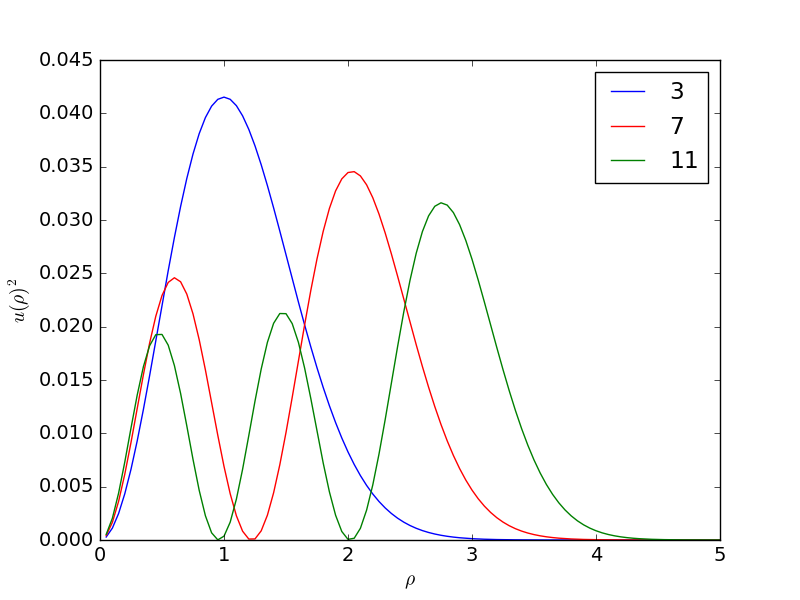
\includegraphics[scale=0.7]{../Programs/Output/Eigenvectors_1pHO.png}
\caption{The eigenvectors corresponding to the three lowest eigenstates.}
\label{fig:eigenvectors_1p}
\end{center}
\end{figure}



\subsection{Two-particle case}

\section{Summary and conclusions}

\begin{thebibliography}{40}

\bibitem{Matrix Comp} G. Golub, C. Van Loan (1996), \textit{Matrix Computations}, John Hopkins University 
Press. 

\bibitem{Lecture Notes} M. Hjort-Jensen (2015), \textit{Computational Physics - Lecture Notes Fall 2015}, 
Department of Physics, University of Oslo. \\ 
\href{https://github.com/CompPhysics/ComputationalPhysics/blob/master/doc/Lectures/lectures2015.pdf}
{https://github.com/CompPhysics/ComputationalPhysics/blob/master\\/doc/Lectures/lectures2015.pdf}

\bibitem{Lectures Eigenvalue Problems} M. Hjort-Jensen (2017), \textit{Computational Physics Lectures: 
Eigenvalue Problems}. 
\href{http://compphysics.github.io/ComputationalPhysics/doc/pub/eigvalues/pdf/eigvalues-beamer.pdf}
{http://compphysics.github.io/ComputationalPhysics/doc/pub/eigvalues\\/pdf/eigvalues-beamer.pdf}

\end{thebibliography}

\end{document}
